% generated by src/r2/paper_assets (make_paper_assets.py figures); do not edit by hand
% provenance: figS4_gov_grid generated by src/r2/paper_assets on 2026-10-15 04:07 from data/r2/tables/
%   gov_sensitivity_grid.csv (modified 2026-10-14 20:11): family == 'q_grid' (dual_rule primary) and family == 'dual_rule' (primary, lenient, strict); reference in (encode, enets2, pert_pooled); columns n_promoted, n_strong, oe_tf, oe_tf_lo, oe_tf_hi
\begin{figure}[htbp]
  \centering
  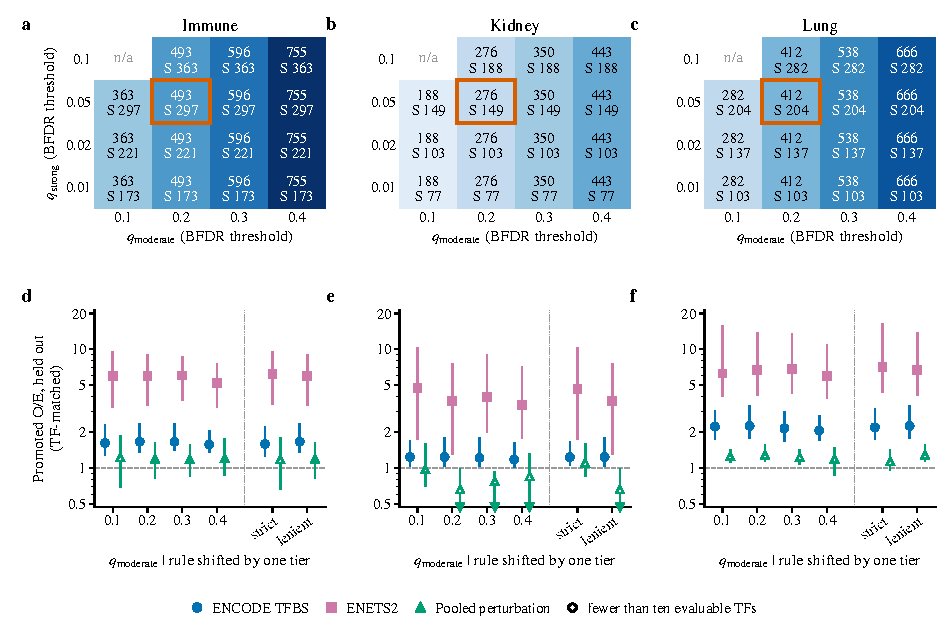
\includegraphics[width=\textwidth]{figS4_gov_grid.pdf}
  \caption{\textbf{Sensitivity of claim governance to the BFDR thresholds} (dual-universe rule). (a--c) Number of promoted edges (Strong $\cup$ Moderate; colour and upper number) and of Strong edges (S) over the grid of $q_\mathrm{strong} \times q_\mathrm{moderate}$; the prespecified point is outlined. Under the primary rule $q_\mathrm{strong}$ only moves edges between Strong and Moderate, so the promoted set and its enrichment do not depend on it (largest change of O/E across $q_\mathrm{strong}$: 0.00). (d--f) Observed over TF-matched expected held-out positives in the promoted set, by $q_\mathrm{moderate}$ at the prespecified $q_\mathrm{strong}$, and for the rules shifted by one tier (strict, lenient) at the prespecified thresholds; bars: 95\% TF-cluster bootstrap intervals (triangles: lower limit below the axis range); open markers: intervals resting on fewer than ten evaluable TFs; reference line at 1.}
  \label{fig:S-gov-grid}
\end{figure}
